\documentclass[10pt,a4paper]{article}
\usepackage[latin1]{inputenc}
\usepackage{amsmath}
\usepackage{amsfonts}
\usepackage{amssymb}
\usepackage{graphicx}
\begin{document}
	from this we know where the decays are happening.
	
	Assuming the following quantities (TODO add pdg data link oder wikipedia link):
	[TODO find values]
	[TODO show gamma, beta claculation...]

%	MASSEN
	
%	mK+ = (493.677�0.016) * 10**6 eV
%	http://pdg.lbl.gov/2017/listings/rpp2017-list-K-plus-minus.pdf (1)
%	
%	mpi+ = (139.57061�0.00024) * 10**6 eV 
%	http://pdg.lbl.gov/2017/listings/rpp2017-list-pi-plus-minus.pdf (1)
%	
%	mpi0 = (134.9770�0.0005) * 10**6 eV
%	http://pdg.lbl.gov/2017/listings/rpp2017-list-pi-zero.pdf (1)
	
	\begin{align*}
		m_{K^+} = \\
		m_{pi^+ } =\\
		m_{pi^0 } =\\
		\beta =\\
		\gamma =\\ 
	\end{align*}
	
	In the $K^+$ rest frame we now have a momentum of 0 and a rest energy $m_K^+$. The $K^+$ now decays into a $\pi^+$ and a $\pi^0$ with momenta $p_{\pi^+} $, $p_{\pi^0} $ in oposing directions. The momenta must have the same magnitude and $p_{\pi^+} = -p_{\pi^0} $ .
	
	The magnitude of the momentum is calculated with  the energy of lost mass in the decay. In the following equations $p$ is used as absolute scalar.
		
	\begin{align}
		E_{\pi^+} = \frac{m_{K^+}^2 + m_{pi^+ }^2 - m_{pi^0 }^2 } {2 m_{K^+}}\\
		p_{\pi^+} = \sqrt{E_{\pi^+}^2 - m_{pi^+ }^2 }\\
		p_{\pi^+ } = p_{\pi^0 }\\
	\end{align}

	
	We use isotropically distributed unit vetors in the simulation (see AW). We multiply them with $p_{\pi^0}$ to get the momenta for $\pi^0$ in the $K^+$ rest frame. Tho get the momenta of $\pi^+$ we take the same distribution and flip signs. We then build the four vectors  $P^*_{\pi}$.
	
	\begin{align}
		 P^*_{\pi} = 
		\begin{bmatrix}
				E_{\pi}^* \\ p_{\pi,x}^* \\ p_{\pi,y}^* \\ p_{\pi,z}^*
		\end{bmatrix} = 
		\begin{bmatrix}
				\sqrt{m_{\pi}^2 + ||p_{\pi}||^2 } \\ p_{\pi,x}^* \\ p_{\pi,y}^* \\ p_{\pi,z}^*
		\end{bmatrix}
	\end{align}
	
	Back to the lab rest frame, we boost them with the boost matrix. This boost matrix performs a boost along the z-axis. 
	
	\begin{align}
		P_{\pi} =
		\begin{bmatrix}
		\gamma & 0 & 0 & \beta \gamma \\
		0 & 1 & 0 & 0 \\
		0 & 0 & 1 & 0\\
		\beta \gamma & 0 & 0 & \gamma \\
		\end{bmatrix}
		\cdot
		P^*_{\pi}
	\end{align}
	
		$P_{\pi}$ is the four-vector in the lab frame. $P_{\pi}^*$ is the four-vector in the kaon rest frame. 
	
	\subsection{With scattering}
	
		When we use a beam that is not parallel to the z-axis, we need to perform a rotation to the momentum of the four-vector before and after the boost. The rotation after the boost is the same that would rotate $e_z$ to align with the position vector. the one before is the inverse rotation.
		
		Since the momentum of the four-vectors $P_{\pi}$ of the pions are isotropically distributed in the  $K^+$ rest frame, we can omit the first rotation and still end up with a an isotropical distribution.
		
		The operation performed with the angle $\alpha$ around y-axis and $\beta$ around x-axis:
		
		\begin{align}
				R(\alpha, \beta) = \begin{bmatrix}
				\cos \alpha  & 0 & \sin \alpha \\
				0         & 1 &  0          \\
				-\sin \alpha & 0 & \cos \alpha
				\end{bmatrix} \cdot \begin{bmatrix}
				1 &   0         & 0           \\
				0 & \cos \beta & -\sin \beta \\
				0 & \sin \beta &  \cos \beta
				\end{bmatrix}
		\end{align}
		
		We apply $R(\alpha, \beta)$ to the momentum after we have extracted	the momentum of the four-vector $P_{\pi}$.
		
		\section{Hits}
		\label{hits}
		
		To determine the number of decays for which both pions hit the detector, we first define a distance $z_d$ from source to detector. And a radius $r$ of the detector. The impulses in the lab frame are $\overrightarrow{p_{\pi^+}}$ and $\overrightarrow{p_{\pi^0}}$. And decay position $\overrightarrow{x} = (x, y, z)$. We want to find the number of double hits.
				
		\begin{enumerate}
			\item Drop all the decay entries where $z > z_d$.
			\item Do the following for $\overrightarrow{p} = \overrightarrow{p_{\pi^+}}$ or $\overrightarrow{p_{\pi^0}}$.
			\begin{enumerate}
				\item Calculate $s$ such that $\overrightarrow{q} = \overrightarrow{x} + s \cdot \overrightarrow{p}$ lands in the plane of $z_d$.
				\item Drop the pion if it's outside the detector. $ (x + q_x)^2 + (y + q_y)^2 > r^2$. % code 1
			\end{enumerate}
			\item Drop the decay if at least one of the two pions was dropped.
			\item Count the number of decays left. % code  2
		\end{enumerate}
	
	% code 2 TODO: reference code file...
%	def single_hit(decay_position, four_vecs, z_detector, detector_radius):
%	"""check if one particle hit the detector"""
%	p = four_vecs[:, 1:]
%	x, y, z = decay_position.T
%	
%	# q is the position the particle will pass in the plane through z_detector
%	q = p.T * (-z + z_detector) / p[:,2]
%	qx, qy, qz = q
%	
%	# return whether the particles hit the circular disk
%	return (x + qx)**2 + (y + qy)**2 > detector_radius**2
	
		% code 2
%		def count_double_hits(decay_positions, particle1_4vec, particle2_4vec, r, z_detector):
%		"""count for how many of the decays, particle1 and particle2 hit the detector"""
%		
%		# numpy filter to filter the ones that decay in front of the detector
%		in_front = decay_positions[:,2] < z_detector
%		
%		# drop the decays that are behind
%		decay_positions = decay_positions[in_front]
%		particle1_4vec = particle1_4vec[in_front]
%		particle2_4vec = particle2_4vec[in_front]
%		
%		# boolean array. True if hit, False if miss
%		hits1 = single_hit(decay_positions, particle1_4vec, z_detector, r)
%		hits2 = single_hit(decay_positions, particle2_4vec, z_detector, r)
%		
%		# combine the with elementwise and.
%		hits = hits1 & hits2
%		return len(decay_positions[hits])

	
\section{Determine The optimal detector distance $z_d$}
	We will now determine the optimal distance such that the acceptance of is maximized. Acceptance is defined as follows:
	
	\begin{align}
		P(z_d) = \frac{\text{n decays for which both pions hit}}{\text{n decays simulated}} 
	\end{align}
	
	To maximize the acceptance we run the experiment about 500 times with $N = 10^6 $ kaons generated. First we simulate a beam aligned to the z axis. Second we generate a beam that scatters at the source in a gaussian distribution with $\sigma _{\theta} = 0.001$ rad.
	
	To determine the optimal z distance, we implemented the algorithm described in \ref{hits}. We let it run for z values in a range from 215 to 350 meters in 85 evenly sized steps. The algorithm generates 85 double hit counts in an array. We divide by N to get the probabilities. Then we fit it with a polynom of degree 3 and determine the maximum of that polynom. To show it graphically, we will show a plot. The simulation was run once with $N = 10^6 $ decays.
	
\begin{figure}
	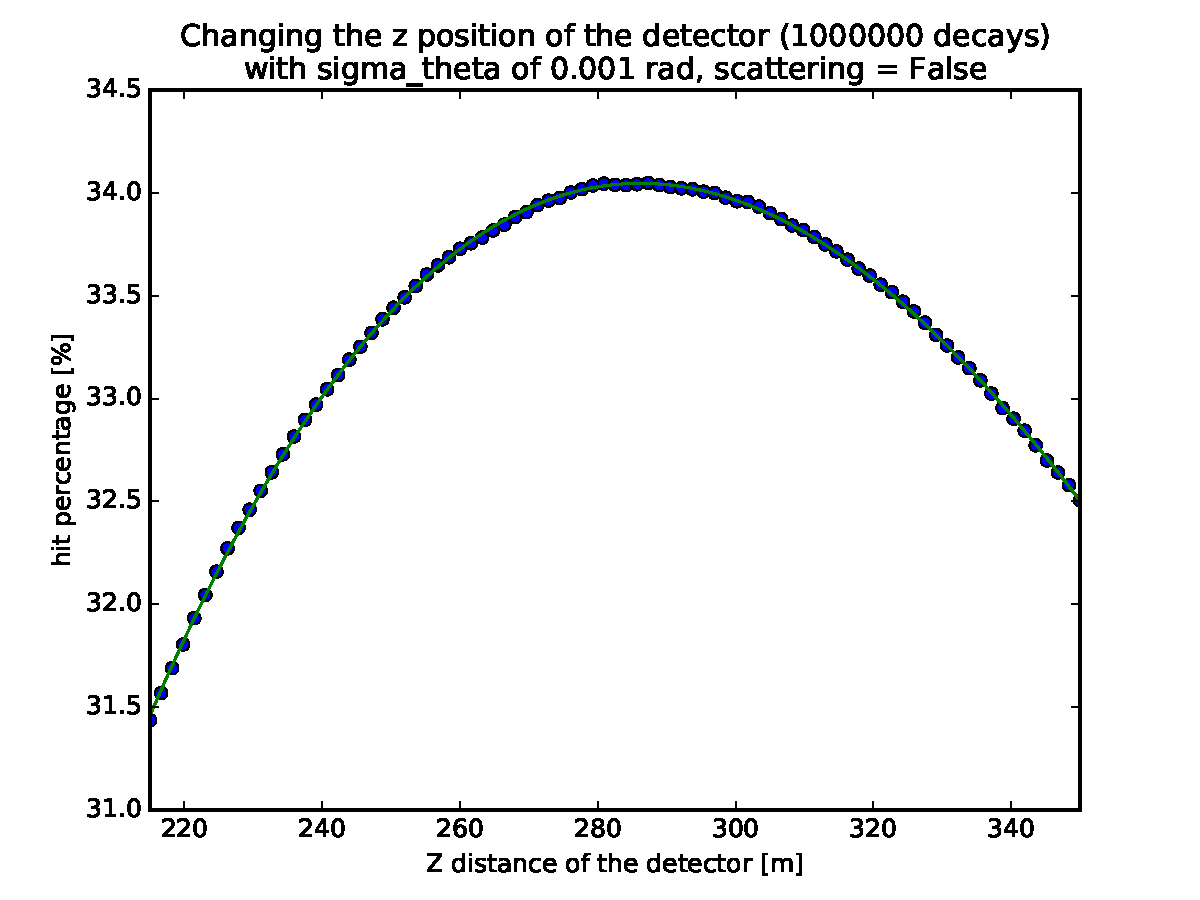
\includegraphics[width=\linewidth]{sample_figure_1000000.pdf}
	\caption{Sample output of decay\_simulation\_6.py}
	\label{fig:figure1000000215to350in85562}
\end{figure}
	
	We run the simulation about 500 times. Fitting the maximum and saving it. The maxima are then put into a histogram.  the average and standard deviation of the maximas are listed below. The standard deviation gives a measure of the statistical uncertainty of the simulation.
	
	[TODO add units]
	
	\textbf{Aligned Beam}
		\begin{align*}
		 <z> = 285.5\\
		\sigma _z  : 0.7\\
		\end{align*}
	
	\textbf{Scattered Beam}
		\begin{align*}
		<z> = 280.7\\
		\sigma _z  : 0.7\\
		\end{align*}
		
		To calculate the final uncertainty we used the relative error on the average decay length from chapter [TODO add reference]. The relative errors get quadratically added.
		
		\begin{align}
			m_z = \sigma _z \cdot \sqrt{ \left(\frac{\text{uncertanty on adl}}{\text{adl}}\right)^2 +  \left(\frac{\sigma_z}{z}\right)^2}
		\end{align}
		
		The final optimal values for z are:
		
		\begin{align*}
			z_{\text{aligned}} =  (286 \pm 5) m\\
			z_{\text{scattered}} =  (281 \pm 5) m
		\end{align*}
		
		The error does not matter that much, since a change of 5 meters around the maximum does maximally change the acceptance by 0.5 percent as seen in figure \ref{fig:figure1000000215to350in85562}.
		
\begin{figure}
	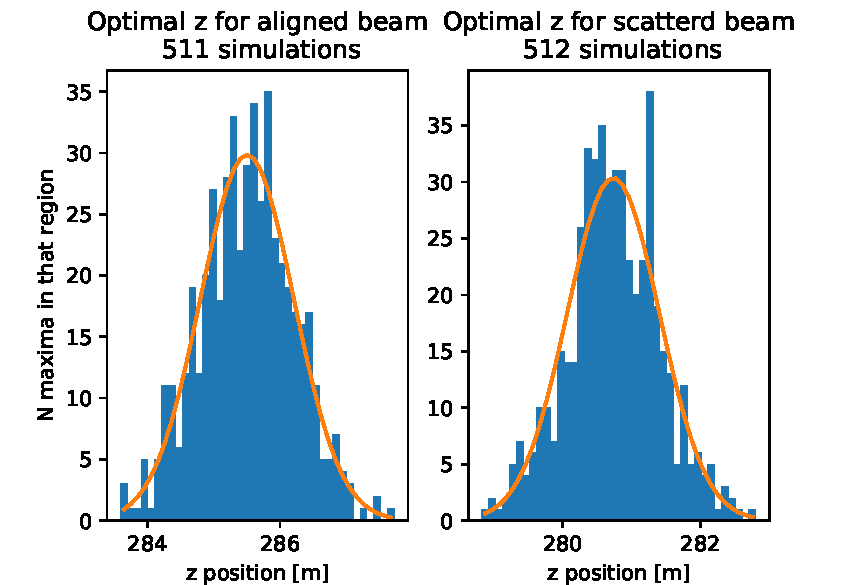
\includegraphics[scale=1]{optimal_zpos.pdf}
	\caption{[TODO find good title]}
	\label{fig:optimalzpos}
\end{figure}
	
	
	
	
	
	
	
	
\end{document}